\documentclass[paperwidth=36in,paperheight=24in,fontscale=0.475]{baposter} % Adjust the font scale/size here
\usepackage{tcolorbox}
\usepackage{xspace}
\usepackage{graphicx} % Required for including images
\graphicspath{{figures/}} % Directory in which figures are stored
\usepackage{subfigure}
\usepackage{amsmath} % For typesetting math
\usepackage{amssymb} % Adds new symbols to be used in math mode
\usepackage{wrapfig}
\usepackage{booktabs} % Top and bottom rules for tables
\usepackage{enumitem} % Used to reduce itemize/enumerate spacing
\usepackage{palatino} % Use the Palatino font
\usepackage[font=small,labelfont=bf]{caption} % Required for specifying captions to tables and figures
\usepackage[makeroom]{cancel}
\usepackage{multicol} % Required for multiple columns
\setlength{\columnsep}{1.5em} % Slightly increase the space between columns
\setlength{\columnseprule}{0mm} % No horizontal rule between columns
\usepackage{xcolor}
\usepackage{tikz} % Required for flow chart
\usetikzlibrary{automata,positioning,arrows} % Tikz libraries required for the flow chart in the template
\usepackage{agda}
\renewcommand{\AgdaBoundFontStyle}[1]{\texttt{#1}}
\usepackage[T1]{fontenc}
\usepackage{unicode-math}
\setmathfont{XITS Math}
\usepackage{thesis-shortcuts}
\usepackage{thesis-unicode}

\newcommand{\compresslist}{ % Define a command to reduce spacing within itemize/enumerate environments, this is used right after \begin{itemize} or \begin{enumerate}
\setlength{\itemsep}{1pt}
\setlength{\parskip}{0pt}
\setlength{\parsep}{0pt}
}
\definecolor{maroon}{HTML}{800035}
\definecolor{lightblue}{rgb}{0.145,0.6666,1} 
\definecolor{pastelyellow}{rgb}{0.958,0.958, 0.535}
\definecolor{blues}{HTML}{B1F1E6}
\definecolor{greens}{rgb}{0.538,0.925,0.610}

\newcommand{\U}{\mathbf{U}}
\newcommand{\F}{\mathbf{F}}
\newcommand{\G}{\mathbf{G}}
\newcommand{\X}{\mathbf{X}}
\newcommand{\BK}{\mathcal{BK}}
 \newcommand{\HyperLTL}{HyperLTL\xspace}
 \newcommand{\hilight}[1]{\colorbox{pastelyellow}{#1}}
\newcommand{\hilightred}[1]{\colorbox{red}{#1}}
\newcommand{\hilightlg}[1]{\colorbox{blues}{#1}}
\setlength{\columnsep}{0.2cm}
\newcommand\enrec[1]{%
  \tikz[baseline=(X.base)]
    \node (X) [draw, shape=rectangle, inner sep=0, fill=white] {\strut #1};}

\newcommand\encirclew[1]{%
  \tikz[baseline=(X.base)]
    \node (X) [draw, shape=circle, inner sep=0, fill=white] {\strut #1};}

\newcommand\encirclegr[1]{%
  \tikz[baseline=(X.base)]
    \node (X) [draw, shape=circle, inner sep=0, fill=gray] {\strut #1};}

 \newcommand\encirclep[1]{%
  \tikz[baseline=(X.base)]
    \node (X) [draw, shape=circle, inner sep=0, fill=pink] {\strut #1};}

\newcommand\encircle[1]{%
  \tikz[baseline=(X.base)]
    \node (X) [draw, shape=circle, inner sep=0, fill=greens] {\strut #1};}

\newcommand\encircley[1]{%
  \tikz[baseline=(X.base)]
    \node (X) [draw, shape=circle, inner sep=0, fill=pastelyellow] {\strut #1};}

\newcommand\encircler[1]{%
  \tikz[baseline=(X.base)]
    \node (X) [draw, shape=circle, inner sep=0, fill=red] {\strut #1};}

\begin{document}

\begin{poster}
{
headerborder=closed, % Adds a border around the header of content boxes
colspacing=1em, % Column spacing
bgColorOne=white, % Background color for the gradient on the left side of the poster
bgColorTwo=white, % Background color for the gradient on the right side of the poster
borderColor=gray, % Border color
headerColorOne=maroon, % Background color for the header in the content boxes (left side)
headerColorTwo=maroon, % Background color for the header in the content boxes (right side)
headerFontColor=white, % Text color for the header text in the content boxes
boxColorOne=white, % Background color of the content boxes
textborder=roundedleft, % Format of the border around content boxes, can be: none, bars, coils, triangles, rectangle, rounded, roundedsmall, roundedright or faded
eyecatcher=true, % Set to false for ignoring the left logo in the title and move the title left
headerheight=0.16\textheight, % Height of the header
headershape=roundedright, % Specify the rounded corner in the content box headers, can be: rectangle, small-rounded, roundedright, roundedleft or rounded
headerfont=\Large\bf\textsc, % Large, bold and sans serif font in the headers of content boxes
%textfont={\setlength{\parindent}{1.5em}}, % Uncomment for paragraph indentation
linewidth=2pt % Width of the border lines around content boxes
}
%----------------------------------------------------------------------------------------
%	TITLE SECTION 
%----------------------------------------------------------------------------------------
%
{
\includegraphics[height=10em]{mac2.png}} % First university/lab logo on the left
{\bf\textsc{Formalising automata theory in Agda}} % Poster title
{\textsc{Mark Armstrong \hspace{12pt} \\ Department of Computing And Software, McMaster University
\\ \vspace{4pt} Supervisors: Jeffery Zucker \& Wolfram Kahl  \vspace{-5pt}}} % Author names and institution
{
\includegraphics[height=9em]{cas.png}} % Second university/lab logo on the right



\headerbox{Problem: Formalising automata theory}{name=problem,column=0,row=0}{
  By \emph{formalise} we mean to \emph{mechanise} in an automated
  proof assistant.

  ~
  
  Sub-problems:
  \begin{itemize}
  \item Create representations of automata
  \item Code their semantics
  \item Complete formal proofs of known properties; e.g.
    \begin{itemize}
    \item computational (in)equivalence of various machines
    \item closure properties (of languages accepted)
    \item existence of minimal state machines
    \end{itemize}
  \end{itemize}

  ~
  
  End goal is to formalise \emph{generalised computability theory},
  meaning computation on \emph{any} ring, e.g.~the real numbers.
}



\headerbox{Motivation}{name=motivation,column=0,below=problem}{
  Formalisation (mechanisation):
  \begin{itemize}
  \item Promotes careful inspection of existing (by-hand) work
  \item Provides \emph{algorithms}
    \begin{itemize}
    \item We work in tools which are founded on \emph{constructive} mathematics
    \item A constructive proof \emph{is an algorithm}
    \end{itemize}
  \item Is intellectually satisfying :)
  \end{itemize}

  ~

  There are existing formalisations in various languages, but they have
  narrow scope.
  \begin{itemize}
  \item Work with just a few machines.
  \item 
  \end{itemize}
}



\headerbox{Methodology: Proofs $\approx$ Programs}{name=methodology,column=0,below=problem}{
  \begin{itemize}
  \item Agda is a dependently typed programming language.
  \item By the Curry-Howard correspondence, \emph{propositions}
    correspond to \emph{types}.
  \item So an Agda type can be viewed as a proposition.
  \end{itemize}
  
  Examples:
  \begin{itemize}
  \item \AgArg{n} : \AgDT{ℕ}
    \begin{itemize}
    \item Proof there is a natural number
    \end{itemize}
  \item (\AgArg{n} : \AgDT{ℕ})\; →\; \AgArg{n} \AgDT{<} \AgIC{suc} \AgArg{n}
    \begin{itemize}
    \item Proof every natural is less than its successor
    \end{itemize}
  \item \AgArg{p?} : \AgFun{Decidable} \AgArg{P}
    \begin{itemize}
    \item Proof that a predicate \AgArg{P} is decidable;
      i.e.~\AgArg{p?} is a decision procedure for \AgArg{P}
    \end{itemize}
  \end{itemize}
}




\headerbox{A representation of deterministic finite automata}{name=dfas,column=1}{
  \begin{code}%
    \>[0]\AgdaKeyword{record}\AgdaSpace{}%
    \AgdaRecord{DFA}\AgdaSpace{}%
    \AgdaSymbol{(}\AgdaBound{|Σ|}\AgdaSpace{}%
    \AgdaSymbol{:}\AgdaSpace{}%
    \AgdaDatatype{ℕ}\AgdaSymbol{)}\AgdaSpace{}%
    \AgdaSymbol{:}\AgdaSpace{}%
    \AgdaPrimitiveType{Set₁}\AgdaSpace{}%
    \AgdaKeyword{where}\<%
    \\
    \>[0][@{}l@{\AgdaIndent{0}}]%
    \>[2]\AgdaKeyword{constructor}\AgdaSpace{}%
    \AgdaOperator{\AgdaInductiveConstructor{⟨\AgdaUnderscore{},\AgdaUnderscore{},\AgdaUnderscore{},\AgdaUnderscore{}⟩}}\<%
    \\
    %
    \>[2]\AgdaKeyword{field}\<%
    \\
    \>[2][@{}l@{\AgdaIndent{0}}]%
    \>[4]\AgdaField{|Q|}\AgdaSpace{}%
    \AgdaSymbol{:}\AgdaSpace{}%
    \AgdaDatatype{ℕ}\<%
    \\
    \>[0]\<%
    \\
    %
    \>[2]\AgdaFunction{Q}\AgdaSpace{}%
    \AgdaSymbol{:}\AgdaSpace{}%
    \AgdaPrimitiveType{Set}\<%
    \\
    %
    \>[2]\AgdaFunction{Q}\AgdaSpace{}%
    \AgdaSymbol{=}\AgdaSpace{}%
    \AgdaDatatype{Fin}\AgdaSpace{}%
    \AgdaField{|Q|}\<%
    \\
    %
    \\[\AgdaEmptyExtraSkip]%
    %
    \>[2]\AgdaFunction{Σ}\AgdaSpace{}%
    \AgdaSymbol{:}\AgdaSpace{}%
    \AgdaPrimitiveType{Set}\<%
    \\
    %
    \>[2]\AgdaFunction{Σ}\AgdaSpace{}%
    \AgdaSymbol{=}\AgdaSpace{}%
    \AgdaDatatype{Fin}\AgdaSpace{}%
    \AgdaBound{|Σ|}\<%
    \\
    %
    \\[\AgdaEmptyExtraSkip]%
    %
    \>[2]\AgdaKeyword{field}\<%
    \\
    \>[2][@{}l@{\AgdaIndent{0}}]%
    \>[4]\AgdaField{s}\AgdaSpace{}%
    \AgdaSymbol{:}\AgdaSpace{}%
    \AgdaFunction{Q}\<%
    \\
    %
    \>[4]\AgdaSymbol{\{}\AgdaField{F}\AgdaSymbol{\}}\AgdaSpace{}%
    \AgdaSymbol{:}\AgdaSpace{}%
    \AgdaFunction{PredicateOn}\AgdaSpace{}%
    \AgdaFunction{Q}\<%
    \\
    %
    \>[4]\AgdaField{F?}\AgdaSpace{}%
    \AgdaSymbol{:}\AgdaSpace{}%
    \AgdaFunction{Decidable}\AgdaSpace{}%
    \AgdaField{F}\<%
    \\
    %
    \>[4]\AgdaField{δ}\AgdaSpace{}%
    \AgdaSymbol{:}\AgdaSpace{}%
    \AgdaFunction{Q}\AgdaSpace{}%
    \AgdaSymbol{→}\AgdaSpace{}%
    \AgdaFunction{Σ}\AgdaSpace{}%
    \AgdaSymbol{→}\AgdaSpace{}%
    \AgdaFunction{Q}\<%
  \end{code}
}



\headerbox{Encoding of semantics}{name=dfa-semantics,column=1,below=dfas}{
  \begin{itemize}
  \item Transitive closure of the transition function:
    \begin{code}%
      \>[0]\AgdaFunction{δ*}%
      \>[454I]\AgdaSymbol{:}\AgdaSpace{}%
      \AgdaSymbol{(}\AgdaBound{M}\AgdaSpace{}%
      \AgdaSymbol{:}\AgdaSpace{}%
      \AgdaRecord{DFA}\AgdaSpace{}%
      \AgdaGeneralizable{|Σ|}\AgdaSymbol{)}\AgdaSpace{}%
      \AgdaSymbol{→}\AgdaSpace{}%
      \AgdaFunction{Q}\AgdaSpace{}%
      \AgdaSymbol{→}\AgdaSpace{}%
      \AgdaDatatype{String}\AgdaSpace{}%
      \AgdaFunction{Σ}\AgdaSpace{}%
      \AgdaSymbol{→}\AgdaSpace{}%
      \AgdaFunction{Q}\<%
      \\
      \>[0]\AgdaFunction{δ*}\AgdaSpace{}%
      \AgdaBound{M}\AgdaSpace{}%
      \AgdaBound{q}\AgdaSpace{}%
      \AgdaInductiveConstructor{[]}\AgdaSpace{}%
      \AgdaSymbol{=}\AgdaSpace{}%
      \AgdaBound{q}\<%
      \\
      \>[0]\AgdaFunction{δ*}\AgdaSpace{}%
      \AgdaBound{M}\AgdaSpace{}%
      \AgdaBound{q}\AgdaSpace{}%
      \AgdaSymbol{(}\AgdaBound{x}\AgdaSpace{}%
      \AgdaOperator{\AgdaInductiveConstructor{∷}}\AgdaSpace{}%
      \AgdaBound{xs}\AgdaSymbol{)}\AgdaSpace{}%
      \AgdaSymbol{=}\AgdaSpace{}%
      \AgdaFunction{δ*}\AgdaSpace{}%
      \AgdaBound{M}\AgdaSpace{}%
      \AgdaSymbol{(}\AgdaFunction{δ}\AgdaSpace{}%
      \AgdaBound{q}\AgdaSpace{}%
      \AgdaBound{x}\AgdaSymbol{)}\AgdaSpace{}%
      \AgdaBound{xs}\<%
    \end{code}
  \item Acceptance relation:
    \begin{code}%
      \>[0]\AgdaOperator{\AgdaFunction{\AgdaUnderscore{}Accepts\AgdaUnderscore{}}}%
      \>[532I]\AgdaSymbol{:}\AgdaSpace{}%
      \AgdaSymbol{(}\AgdaBound{M}\AgdaSpace{}%
      \AgdaSymbol{:}\AgdaSpace{}%
      \AgdaRecord{DFA}\AgdaSpace{}%
      \AgdaGeneralizable{|Σ|}\AgdaSymbol{)}\AgdaSpace{}%
      \AgdaSymbol{→}\AgdaSpace{}%
      \AgdaDatatype{String}\AgdaSpace{}%
      \AgdaFunction{Σ}\AgdaSpace{}%
      \AgdaSymbol{→}\AgdaSpace{}%
      \AgdaPrimitiveType{Set}\<%
      \\
      \>[0]\AgdaBound{M}%
      \>[549I]\AgdaOperator{\AgdaFunction{Accepts}}\AgdaSpace{}%
      \AgdaBound{xs}\AgdaSpace{}%
      \AgdaSymbol{=}\AgdaSpace{}%
      \AgdaFunction{F}\AgdaSpace{}%
      \AgdaSymbol{(}\AgdaFunction{δ*}\AgdaSpace{}%
      \AgdaBound{M}\AgdaSpace{}%
      \AgdaFunction{s}\AgdaSpace{}%
      \AgdaBound{xs}\AgdaSymbol{)}\<%
    \end{code}
  \end{itemize}
}



\headerbox{A “general” notion of (deterministic) automata}{name=general,column=1,below=dfa-semantics}{
  We want to be as general as possible --- while still being reasonable.
  \begin{code}%
    \>[0][@{}l@{\AgdaIndent{0}}]%
    \>[2]\AgdaKeyword{record}\AgdaSpace{}%
    \AgdaRecord{Automaton}\AgdaSpace{}%
    \AgdaSymbol{:}\AgdaSpace{}%
    \AgdaPrimitiveType{Set₁}\AgdaSpace{}%
    \AgdaKeyword{where}\<%
    \\
    \>[2][@{}l@{\AgdaIndent{0}}]%
    \>[4]\AgdaKeyword{constructor}\AgdaSpace{}%
    \AgdaOperator{\AgdaInductiveConstructor{⟨\AgdaUnderscore{},\AgdaUnderscore{},\AgdaUnderscore{},\AgdaUnderscore{}⟩}}\<%
    \\
    \>[4]\AgdaKeyword{field}\<%
    \\
    \>[4][@{}l@{\AgdaIndent{0}}]%
    \>[6]\AgdaField{i}\AgdaSpace{}%
    \AgdaSymbol{:}\AgdaSpace{}%
    \AgdaFunction{StateIndex}\<%
    \\
    \>[0]\<%
    \\
    %
    \>[4]\AgdaFunction{Q}\AgdaSpace{}%
    \AgdaSymbol{:}\AgdaSpace{}%
    \AgdaPrimitiveType{Set}\<%
    \\
    %
    \>[4]\AgdaFunction{Q}\AgdaSpace{}%
    \AgdaSymbol{=}\AgdaSpace{}%
    \AgdaFunction{StateSpace}\AgdaSpace{}%
    \AgdaField{i}\<%
    \\
    \>[0]\<%
    \\
    %
    \>[4]\AgdaKeyword{field}\<%
    \\
    \>[4][@{}l@{\AgdaIndent{0}}]%
    \>[6]\AgdaField{s}\AgdaSpace{}%
    \AgdaSymbol{:}\AgdaSpace{}%
    \AgdaFunction{Q}\<%
    \\
    %
    \>[6]\AgdaSymbol{\{}\AgdaField{F}\AgdaSymbol{\}}\AgdaSpace{}%
    \AgdaSymbol{:}\AgdaSpace{}%
    \AgdaFunction{PredicateOn}\AgdaSpace{}%
    \AgdaFunction{Q}\<%
    \\
    %
    \>[6]\AgdaField{F?}\AgdaSpace{}%
    \AgdaSymbol{:}\AgdaSpace{}%
    \AgdaFunction{Decidable}\AgdaSpace{}%
    \AgdaField{F}\<%
    \\
    %
    \>[6]\AgdaField{δ}\AgdaSpace{}%
    \AgdaSymbol{:}\AgdaSpace{}%
    \AgdaFunction{Q}\AgdaSpace{}%
    \AgdaSymbol{→}\AgdaSpace{}%
    \AgdaFunction{Σ}\AgdaSpace{}%
    \AgdaSymbol{→}\AgdaSpace{}%
    \AgdaFunction{Q}\AgdaSpace{}\AgdaDatatype{×}\AgdaSpace{}\AgdaFunction{Action}\<%
  \end{code}

  For instance, a  Turing machine is an \AgdaRecord{Automaton} with a finite \AgdaFunction{Q}
  and actions which manipulate its tape(s).
}



\headerbox{Example proposition: equivalence of DFAs and NFAs}{name=example-prop,column=2}{
  We know \emph{deterministic} and \emph{non-deterministic}
  finite automata are \emph{computationally equivalent} -
  i.e., accept the same languages.

  ~
  
  For instance, an NFA (with two start states)
  which accepts strings of $a$'s whose length is a multiple of 2 or 3.
  \begin{center}
    \fbox{
      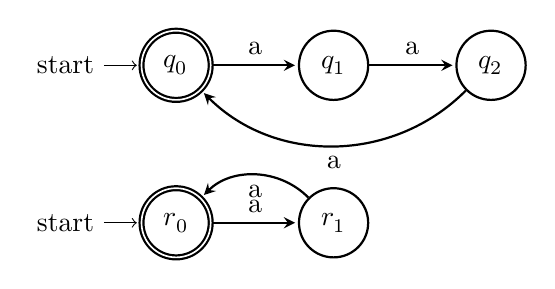
\begin{tikzpicture}[shorten >=1pt,node distance=2cm,on grid,auto] 
        \node[state, initial, accepting, thick] (q_0)                {$q_0$}; 
        \node[state, thick]                     (q_1) [right=of q_0] {$q_1$}; 
        \node[state, thick]                     (q_2) [right=of q_1] {$q_2$}; 
        \node[state, initial, accepting, thick] (r_0) [below=of q_0] {$r_0$};
        \node[state, thick]                     (r_1) [right=of r_0] {$r_1$};
        \path[->, thick, >=stealth] 
        (q_0) edge                   node {a} (q_1)
        (q_1) edge                   node {a} (q_2)
        (q_2) edge [bend left=45]  node {a} (q_0) 
        (r_0) edge                   node {a} (r_1)
        (r_1) edge [bend right=45] node {a} (r_0);
      \end{tikzpicture}
    }
  \end{center}
  And DFA for the same language.
  \begin{center}
    \fbox{
      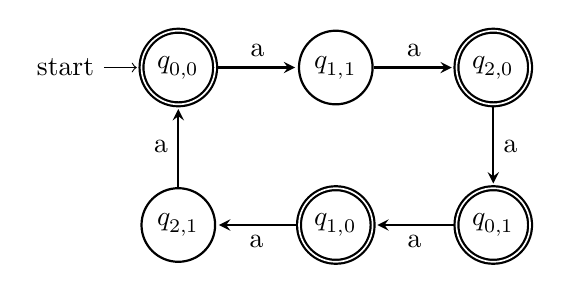
\begin{tikzpicture}[shorten >=1pt,node distance=2cm,on grid,auto] 
        \node[state, initial, accepting, thick] (q00)                {$q_{0,0}$}; 
        \node[state, thick]                     (q11) [right=of q00] {$q_{1,1}$}; 
        \node[state, accepting, thick]          (q20) [right=of q11] {$q_{2,0}$}; 
        \node[state, accepting, thick]          (q01) [below=of q20] {$q_{0,1}$};
        \node[state, accepting, thick]          (q10) [left=of  q01] {$q_{1,0}$};
        \node[state, thick]                     (q21) [left=of  q10] {$q_{2,1}$};
        \path[->, thick, >=stealth] 
        (q00) edge node {a} (q11)
        (q11) edge node {a} (q20)
        (q20) edge node {a} (q01) 
        (q01) edge node {a} (q10)
        (q10) edge node {a} (q21)
        (q21) edge node {a} (q00);
      \end{tikzpicture}
    }
  \end{center}
}



\headerbox{Formalising equivalence of DFAs and NFAs}{name=example-agda,column=2,below=example-prop}{
  In Agda, we formalise (one direction of) this proposition by
  \begin{itemize}
  \item Constructing an NFA for each DFA:
    \begin{code}%
      \>[0]\AgdaFunction{DFA-to-NFA}\AgdaSpace{}%
      \AgdaSymbol{:}\AgdaSpace{}%
      \AgdaRecord{DFA}\AgdaSpace{}%
      \AgdaBound{Σ}\AgdaSpace{}%
      \AgdaSymbol{→}\AgdaSpace{}%
      \AgdaRecord{NFA}\AgdaSpace{}%
      \AgdaBound{Σ}\<%
    \end{code}
  \item Proving it accepts all strings the DFA accepts:
    \begin{code}
      \>[0]\AgdaFunction{accepts{-}all{-}strings}%
      \>[421I]\AgdaSymbol{:}\AgdaSpace{}%
      \AgdaSymbol{(}\AgdaBound{M}\AgdaSpace{}%
      \AgdaSymbol{:}\AgdaSpace{}%
      \AgdaRecord{DFA}\AgdaSpace{}%
      \AgdaBound{|Σ|}\AgdaSymbol{)}\AgdaSpace{}\<%
      \\
      \>[421I][@{}l@{\AgdaIndent{0}}]%
      \>[21]\AgdaSymbol{→}\AgdaSpace{}%
      \AgdaSymbol{(}\AgdaBound{xs}\AgdaSpace{}%
      \AgdaSymbol{:}\AgdaSpace{}%
      \AgdaDatatype{String}\AgdaSpace{}%
      \AgdaFunction{Σ}\AgdaSymbol{)}\<%
      \\
      \>[421I][@{}l@{\AgdaIndent{0}}]%
      \>[21]\AgdaSymbol{→}\AgdaSpace{}%
      \AgdaBound{M}\AgdaSpace{}%
      \AgdaOperator{\AgdaFunction{Accepts}}\AgdaSpace{}%
      \AgdaBound{xs}\<%
      \\
      %
      \>[21]\AgdaSymbol{→}\AgdaSpace{}%
      \AgdaSymbol{(}\AgdaFunction{DFA-to-NFA}\AgdaSpace{}%
      \AgdaBound{M}\AgdaSymbol{)}\AgdaSpace{}%
      \AgdaOperator{\AgdaFunction{Accepts}}\AgdaSpace{}%
      \AgdaBound{xs}\<%
    \end{code}
  \item Proving it accepts \emph{only} the strings the DFA accepts:
    \begin{code}
     \>[0]\AgdaFunction{accepts{-}only{-}strings}%
      \>[421I]\AgdaSymbol{:}\AgdaSpace{}%
      \AgdaSymbol{(}\AgdaBound{M}\AgdaSpace{}%
      \AgdaSymbol{:}\AgdaSpace{}%
      \AgdaRecord{DFA}\AgdaSpace{}%
      \AgdaBound{|Σ|}\AgdaSymbol{)}\AgdaSpace{}\<%
      \\
      \>[421I][@{}l@{\AgdaIndent{0}}]%
      \>[21]\AgdaSymbol{→}\AgdaSpace{}%
      \AgdaSymbol{(}\AgdaBound{xs}\AgdaSpace{}%
      \AgdaSymbol{:}\AgdaSpace{}%
      \AgdaDatatype{String}\AgdaSpace{}%
      \AgdaFunction{Σ}\AgdaSymbol{)}\<%
      \\
      %
      \>[21]\AgdaSymbol{→}\AgdaSpace{}%
      \AgdaSymbol{(}\AgdaFunction{DFA-to-NFA}\AgdaSpace{}%
      \AgdaBound{M}\AgdaSymbol{)}\AgdaSpace{}%
      \AgdaOperator{\AgdaFunction{Accepts}}\AgdaSpace{}%
      \AgdaBound{xs}\<%
      \\
      \>[421I][@{}l@{\AgdaIndent{0}}]%
      \>[21]\AgdaSymbol{→}\AgdaSpace{}%
      \AgdaBound{M}\AgdaSpace{}%
      \AgdaOperator{\AgdaFunction{Accepts}}\AgdaSpace{}%
      \AgdaBound{xs}\<%
    \end{code}
  \end{itemize}
}

\headerbox{References}{name=references,column=0,below=methodology}{
  {\small
  \begin{enumerate}[align=left]
  \item[1] Asperti, Andrea and Ricciotti, Wilmer. Formalizing Turing Machines.
  \item[2] Asperti, Andrea and Ricciotti, Wilmer. A formalization of multi-tape Turing machines.
  \item[3] Constable, Robert L. and Jackson, Paul B. and Naumov, Pavel and Uribe, Juan.\\
    Constructively Formalizing Automata Theory.
  \item[4] Ulf Norell. Towards a practical programming language based on dependent type theory.
  \item[5] Xu, Jian and Zhang, Xingyuan and Urban, Christian.\\
    Mechanising Turing Machines and Computability Theory in Isabelle/HOL.
  \end{enumerate}
  }
}

\end{poster}

\end{document}
